% CO5103 Hệ thống thông tin quản lý - Đồ án, slide báo cáo
% Template HCMUT (giống slide CO5135 Big Data). Build: pdflatex main.tex hai lần.
\documentclass[aspectratio=169,11pt]{beamer}

\usepackage[T5]{fontenc}          % T5 cho tiếng Việt
\usepackage[utf8]{inputenc}
\usepackage[vietnamese]{babel}
\usepackage{lmodern}
\usepackage{graphicx}
\usepackage{booktabs}
\usepackage{array}
\newcolumntype{L}[1]{>{\raggedright\arraybackslash}p{#1}}
\usepackage{tikz}
\usetikzlibrary{arrows.meta,positioning,fit,backgrounds,calc}
\usepackage{pgfplots}
\pgfplotsset{compat=1.17}
\pgfkeys{/pgf/number format/.cd,use comma,1000 sep={.}}  % 10.564 ; 73,6

% ---------------- Theme (HCMUT Beamer template) ----------------
\usetheme{default}
\useinnertheme{circles}
\setbeamertemplate{itemize items}[ball]
\setbeamertemplate{enumerate items}[ball]
\setbeamertemplate{navigation symbols}{}

\definecolor{bkblue}{HTML}{1E4E79}
\definecolor{bkmid}{HTML}{163A5B}
\definecolor{bkdark}{HTML}{0F273C}
\definecolor{bklight}{HTML}{3A9AD9}
\definecolor{bkorange}{HTML}{C8742E}
\definecolor{bkgreen}{HTML}{1F7A3A}
\definecolor{bkgray}{HTML}{8A97A6}

\setbeamercolor{structure}{fg=bkblue}
\setbeamercolor{frametitle}{bg=bkblue,fg=white}
\setbeamercolor{framesubtitle}{fg=white}
\setbeamercolor{title}{fg=bkblue}
\setbeamercolor{block title}{bg=bkblue,fg=white}
\setbeamercolor{block body}{bg=bkblue!8}
\setbeamercolor{block title alerted}{bg=bkorange,fg=white}
\setbeamercolor{block body alerted}{bg=bkorange!10}
\setbeamercolor{block title example}{bg=bkgreen,fg=white}
\setbeamercolor{block body example}{bg=bkgreen!8}
\setbeamerfont{frametitle}{size=\Large}
\setbeamerfont{framesubtitle}{size=\scriptsize}
\setbeamerfont{block title}{size=\small,series=\bfseries}
\setbeamerfont{footnote}{size=\tiny}

\makeatletter
\setbeamertemplate{frametitle}{%
  \nointerlineskip
  \begin{beamercolorbox}[wd=\paperwidth,sep=0.35em,leftskip=0.3em]{frametitle}
    \usebeamerfont{frametitle}\strut\insertframetitle\strut\par
    \ifx\insertframesubtitle\@empty\else
      {\usebeamerfont{framesubtitle}\insertframesubtitle\par}%
    \fi
  \end{beamercolorbox}
}
\makeatother

\setbeamertemplate{footline}{%
  \leavevmode\hbox{%
  \begin{beamercolorbox}[wd=.38\paperwidth,ht=2.4ex,dp=1ex,left,leftskip=0.6em]{author in head/foot}%
    \usebeamerfont{author in head/foot}\insertshortauthor\ (\insertshortinstitute)
  \end{beamercolorbox}%
  \begin{beamercolorbox}[wd=.31\paperwidth,ht=2.4ex,dp=1ex,center]{title in head/foot}%
    \usebeamerfont{title in head/foot}\insertshorttitle
  \end{beamercolorbox}%
  \begin{beamercolorbox}[wd=.31\paperwidth,ht=2.4ex,dp=1ex,right,rightskip=0.6em]{date in head/foot}%
    \usebeamerfont{date in head/foot}\insertshortdate\hspace{2em}\insertframenumber{} / \inserttotalframenumber
  \end{beamercolorbox}}%
  \vskip0pt%
}
\setbeamercolor{author in head/foot}{bg=bkdark,fg=white}
\setbeamercolor{title in head/foot}{bg=bkmid,fg=white}
\setbeamercolor{date in head/foot}{bg=bkblue,fg=white}
\setbeamerfont{author in head/foot}{size=\tiny,series=\bfseries}
\setbeamerfont{title in head/foot}{size=\tiny,series=\bfseries}
\setbeamerfont{date in head/foot}{size=\tiny,series=\bfseries}

\usebackgroundtemplate{
\includegraphics[width=\paperwidth,height=\paperheight]{figures/bg_frame.png}}

% Tiện ích
\newcommand{\good}[1]{\textcolor{bkgreen}{\textbf{#1}}}
\newcommand{\bad}[1]{\textcolor{bkorange}{\textbf{#1}}}

\graphicspath{{figures/}{../figures/}{../figures/tien_do_2/}}

\title[Tác nhân lập lịch sản xuất hợp lý]{Xây dựng tác nhân lập lịch sản xuất tạo ra lịch hợp lý,\\ứng dụng trong ngành sản xuất linh kiện\\[2pt]{\normalsize Trường hợp nghiên cứu: sản xuất bánh xe}}
\author[Võ Văn Dũng]{Võ Văn Dũng (2570708)}
\institute[HCMUT]{Trường Đại học Bách khoa -- ĐHQG TP.HCM}
\date[11/2026]{TP. Hồ Chí Minh, tháng 11/2026}
\newcommand{\course}{Đồ án môn học CO5103 -- Hệ thống thông tin quản lý}
\newcommand{\supervisor}{PGS.TS Võ Thị Ngọc Châu}
\newcommand{\emails}{\texttt{dung.vovan@hcmut.edu.vn}}

\begin{document}

% =====================================================================
{
\usebackgroundtemplate{
\includegraphics[width=\paperwidth,height=\paperheight]{figures/bg_title.png}}
\setbeamertemplate{footline}{}
\begin{frame}[plain]
  \centering
  \vspace{-0.2em}
  
\includegraphics[height=1.15cm]{figures/logo_vnu.png}\hspace{0.6cm}%
  
\includegraphics[height=1.15cm]{figures/logo_bk.png}\par
  \vspace{0.5em}
  {\usebeamercolor[fg]{title}\large\inserttitle\par}
  \vspace{0.5em}
  {\footnotesize\course\par}
  \vspace{0.5em}
  {\small\textbf{Giảng viên hướng dẫn: \supervisor}\par}
  \vspace{0.3em}
  {\small\textbf{Học viên: \insertauthor}\par}
  \vspace{0.4em}
  {\scriptsize\emails\par}
  \vspace{0.4em}
  {\small\insertdate\par}
  \vfill
  
\includegraphics[height=0.55cm]{figures/footer_text.png}
\end{frame}
}

\begin{frame}{Nội dung}
\tableofcontents
\end{frame}

% =====================================================================
\section{Bài toán}

\begin{frame}{Bối cảnh và phát biểu bài toán}
\framesubtitle{Lập lịch sản xuất ở nhà máy linh kiện vẫn nằm trong các file Excel rời rạc}
\begin{columns}[T]
\begin{column}{0.47\textwidth}
\begin{block}{Hiện trạng}
\scriptsize
\begin{itemize}\setlength{\itemsep}{0.25em}
  \item Đơn hàng, tồn kho, tình trạng máy nằm ở \textbf{nhiều file Excel}, lệch phiên bản giữa các bộ phận.
  \item Logic xếp lịch nằm trong kinh nghiệm cá nhân: \textbf{``hộp đen''} với ban lãnh đạo.
  \item Đơn gấp chen ngang phải dò và sửa tay; khó chuẩn hoá, khó mở rộng.
  \item Nhiều ràng buộc cùng lúc: máy điểm nghẽn, setup theo trình tự, khuôn và bảo trì,
        cỡ lô, tồn kho, ca đã mở phải được tận dụng.
\end{itemize}
\end{block}
\end{column}
\begin{column}{0.49\textwidth}
\begin{block}{Tác nhân lập lịch cần}
\scriptsize
\begin{enumerate}\setlength{\itemsep}{0.25em}
  \item Tự động sinh lịch tối ưu hoặc gần tối ưu từ đơn hàng và ràng buộc thực tế.
  \item Tạo \textbf{lịch hợp lý}: tuân thủ đủ ràng buộc vật lý/nghiệp vụ, cân đối có căn cứ giữa
        hạn giao, hiệu suất máy, tồn kho, để lãnh đạo \textbf{tin dùng mà không phải rà tay lại}.
  \item Phản ứng với gián đoạn (đơn gấp, dừng máy): giải lại và so với lịch gốc.
  \item Tận dụng máy trong mỗi ca đã bật, giảm lãng phí nhân công và điện.
\end{enumerate}
\end{block}
\end{column}
\end{columns}
\end{frame}

\begin{frame}{Phạm vi: dây chuyền vành xe 5 công đoạn}
\framesubtitle{Rút gọn từ quy trình thực tế 19 công đoạn của một nhà máy vành hợp kim nhôm}
\centering
\begin{tikzpicture}[font=\scriptsize,
  st/.style={draw=bkblue,fill=bkblue!8,rounded corners=2pt,align=center,minimum height=1.35cm,text width=1.95cm},
  bn/.style={st,draw=bkorange,fill=bkorange!15,thick},
  inv/.style={align=center,font=\tiny,text=bkgray,inner sep=1pt},
  a/.style={-{Stealth[length=4pt]},bkblue,thick},
  pt/.style={draw=bkblue,fill=bkblue!3,rounded corners=2pt,align=center,minimum height=1.0cm},
  node distance=0.85cm]
  \node[st] (c) {\textbf{Đúc}\\CAST\_1, CAST\_2\\lượt 16 vành\\4 khuôn dùng chung};
  \node[bn,right=of c] (h) {\textbf{Nhiệt luyện}\\HT\_1, HT\_2\\mẻ 24 vành, 8 giờ\\\textbf{điểm nghẽn}};
  \node[st,right=of h] (m) {\textbf{Gia công CNC}\\CNC\_1, CNC\_2\\lượt 20 vành};
  \node[st,right=of m] (p) {\textbf{Sơn}\\PAINT\_1, lượt 25\\setup bạc$\to$đen 12',\\đen$\to$bạc 24'};
  \node[st,right=of p] (q) {\textbf{Thử nghiệm}\\\textbf{\& đóng gói}\\QC\_1, lượt 20};
  \foreach \x/\y in {c/h,h/m,m/p,p/q} {\draw[a] (\x) -- node[inv,above=1pt]{kho\\BTP} (\y);}
  % planning tier
  \node[pt,text width=3.0cm,below=1.0cm of c.south west,anchor=north west] (o) {\textbf{Đơn hàng tháng/quý}\\mã, số lượng, hạn giao, ưu tiên};
  \node[pt,text width=3.3cm,right=0.8cm of o] (pl) {\textbf{Tầng kế hoạch}\\tổng hợp nhu cầu theo kỳ 2 tuần\\(Hax \& Meal, 1975)};
  \node[pt,text width=4.2cm,fill=bkblue!20,right=0.8cm of pl] (sc) {\textbf{Tầng lập lịch (trọng tâm đồ án)}\\lượt nào chạy trên máy nào, lúc nào,\\theo thứ tự nào};
  \draw[a] (o)--(pl); \draw[a] (pl)--(sc);
  \draw[a,dashed] (sc.north) -- node[inv,right=2pt]{xếp lịch cho dây chuyền} (sc.north |- c.south);
\end{tikzpicture}
\vspace{0.4em}

\scriptsize 2 dòng sản phẩm (bánh trước F, bánh sau R) $\times$ 2 màu (bạc, đen) $\cdot$ 3 ca/ngày, lò nhiệt luyện chạy 24/7 $\cdot$
dừng máy theo kế hoạch $\cdot$ tồn an toàn, sức chứa kho $\cdot$ thông số là \textbf{ước tính có ghi giả định}, không phải số đo của nhà máy.
\end{frame}

% =====================================================================
\section{Cơ sở lý thuyết và nghiên cứu liên quan}

\begin{frame}{Cơ sở lý thuyết}
\framesubtitle{Flexible job-shop có mở rộng thực tế, đa mục tiêu, nhiều nhóm phương pháp giải}
\begin{columns}[T]
\begin{column}{0.48\textwidth}
\begin{block}{Lớp bài toán}
\scriptsize
\begin{itemize}\setlength{\itemsep}{0.2em}
  \item \textbf{FJSP}: chọn máy trong tập máy đủ điều kiện \emph{và} xếp thứ tự; NP-khó
        (Dauzère-Pérès et al., 2024). Mọi sản phẩm cùng thứ tự công đoạn $\Rightarrow$ gần
        \textbf{hybrid flow shop} (Ruiz \& Vázquez-Rodríguez, 2010).
  \item Mở rộng cần có: setup phụ thuộc trình tự (Allahverdi, 2015), tài nguyên phụ (khuôn),
        lô/mẻ theo công đoạn, lịch ca, tồn kho và giao hàng.
\end{itemize}
\end{block}
\vspace{-0.3em}
\begin{block}{Đa mục tiêu}
\scriptsize
\begin{itemize}\setlength{\itemsep}{0.2em}
  \item Tổng có trọng số (cho phép bù trừ) $\cdot$ thứ tự ưu tiên (lexicographic) $\cdot$
        \textbf{Pareto}: tập lịch không bị trội = \textbf{đường đánh đổi}, sinh bằng \textbf{ràng buộc $\varepsilon$}.
  \item Khi trọng số là \emph{chính sách quản lý}, đưa phương án cho người quản lý chọn.
\end{itemize}
\end{block}
\end{column}
\begin{column}{0.49\textwidth}
\scriptsize
\textbf{Các nhóm phương pháp}\par\vspace{0.2em}
\begin{tabular}{@{}L{1.75cm}L{2.0cm}L{2.85cm}@{}}
\toprule
Nhóm & Đại diện & Đặc điểm\\
\midrule
Luật điều độ & FIFO, EDD, SPT & tức thì, dễ hiểu; không nhìn xa\\
Metaheuristic & SA, GA & mở rộng tốt; phụ thuộc seed\\
Quy hoạch ràng buộc & OR-Tools CP-SAT & ràng buộc phức tạp, có \textbf{cận dưới}; chậm khi lớn\\
Lai CP + tìm kiếm & CP-LNS, warm start & CP trên bài toán con\\
Phân rã thời gian & rolling horizon & giải kỳ dài; không thấy xa\\
Học máy & DRL, GNN & nhanh sau huấn luyện; khó giải thích\\
\bottomrule
\end{tabular}
\vspace{0.4em}

\textbf{Tái lập lịch} (Vieira et al., 2003) và \textbf{diễn giải} (đường găng, độ nhạy, phản thực,
XAI cho vận trù học) là lớp hỗ trợ tin tưởng lịch.
\end{column}
\end{columns}
\end{frame}

\begin{frame}{Bảng đối sánh nghiên cứu liên quan}
\framesubtitle{32 tài liệu, 16 tài liệu 2024--2026; trích bảng đối sánh 17 dòng}
\centering\tiny
\setlength{\tabcolsep}{3pt}
\renewcommand{\arraystretch}{1.08}
\begin{tabular}{@{}L{2.95cm}L{1.9cm}L{2.85cm}L{2.85cm}L{1.55cm}L{1.45cm}@{}}
\toprule
Nghiên cứu & Bài toán & Phương pháp & Ràng buộc đặc thù & Diễn giải & Gián đoạn\\
\midrule
Wang \& Chen 2024 (ESWA) & JSP bán dẫn & GA + hậu xử lý XAI & không & có (sau giải) & không\\
Mehdiyev et al.\ 2024 & JSP & dự đoán quy trình + NSGA-II & không & phản thực & what-if\\
Cheng et al.\ 2024 (IEEE Access) & FJSP + khuôn & MODE đa mục tiêu & máy--khuôn, setup khuôn & không & không\\
Ghaleb et al.\ 2021 (JMS) & FJSP động & GA lai & suy giảm máy, bảo trì & không & thời gian thực\\
Lan \& Berkhout 2025 (PyJobShop) & FJSP/JSP/RCPSP & CP-SAT, CP Optimizer & tổng quát & không & không\\
Song et al.\ 2023 (IEEE TII) & FJSP & GNN + DRL & không & không & --\\
Li et al.\ 2025 (ICLR) & FJSP kỳ dài & rolling horizon + học máy & không đặc thù & không & --\\
Echeverria et al.\ 2025 (ESWA) & FJSP động & CP + học sâu & không đặc thù & không & có\\
Nguyễn Hồng Phúc et al.\ 2026 & FJSP + thuê ngoài & mô hình toán + GA & tăng ca, thuê ngoài & không & --\\
\midrule
\textbf{Đề tài này} & \textbf{FJSP 5 công đoạn, 2 tầng} & \textbf{kết hợp} luật + SA/GA + CP-LNS + CP-SAT $\varepsilon$, lọc Pareto, \textbf{người chọn} &
  \textbf{ca, setup trình tự, khuôn + bảo trì, lô theo công đoạn, tồn BTP, tồn an toàn, sức chứa kho} &
  \textbf{đánh đổi, so 2 lịch, lý giải} & \textbf{đơn gấp, dừng máy biết trước}\\
\bottomrule
\end{tabular}
\vspace{0.5em}

\begin{columns}[T]
\begin{column}{0.48\textwidth}
\scriptsize \textbf{Khoảng trống 1.} Đa số chọn \emph{một} thuật toán rồi so với các thuật toán khác;
thực nghiệm cho thấy mỗi thuật toán mạnh ở một vùng.
\end{column}
\begin{column}{0.48\textwidth}
\scriptsize \textbf{Khoảng trống 2.} Đa số trả về \emph{một} lịch theo hàm mục tiêu cố định; trọng số giao hàng/chi phí
là quyết định quản lý, đổi theo từng kỳ.
\end{column}
\end{columns}
\end{frame}

\begin{frame}{Dữ liệu benchmark và dữ liệu thực nghiệm}
\framesubtitle{Benchmark công khai chỉ kiểm tra được lõi job-shop $\Rightarrow$ tự xây thêm dữ liệu nghiệp vụ}
\begin{columns}[T]
\begin{column}{0.5\textwidth}
\scriptsize
\textbf{Bộ dữ liệu công khai (đã tải, kèm giấy phép)}\par\vspace{0.2em}
\begin{tabular}{@{}L{2.7cm}L{1.3cm}L{2.9cm}@{}}
\toprule
Bộ & Quy mô & Vai trò\\
\midrule
Taillard ta01--ta80 & 80 inst. & lõi job-shop (makespan)\\
OR-Library, Lawrence & 82 inst. & như trên\\
Deliktaş et al.\ 2024 & 43 inst. & chọn máy, setup theo họ SP\\
Mota et al.\ 2020 & 3 tệp & tham số thời gian/năng lượng\\
\bottomrule
\end{tabular}
\vspace{0.4em}

Cổng dữ liệu mở: data.gov (chỉ số vĩ mô), data.gov.vn (chưa có), Kaggle (3 ứng viên chưa kiểm chứng):
\textbf{không bộ nào có đủ ca, khuôn dùng chung, tồn BTP, giao hàng theo đơn}.
\end{column}
\begin{column}{0.46\textwidth}
\scriptsize
\textbf{Hai bộ dữ liệu tự xây (sinh bằng chương trình có tham số)}\par\vspace{0.2em}
\begin{tabular}{@{}lrr@{}}
\toprule
 & Bộ 3 ngày & Bộ 2 tuần\\
\midrule
Đơn hàng & 4 & 24\\
Số vành & 108 & 980\\
Lượt sản xuất & 42 & 269\\
Máy / khuôn & 8 / 4 & 8 / 4\\
\bottomrule
\end{tabular}
\vspace{0.4em}
\begin{itemize}\setlength{\itemsep}{0.15em}
  \item Bộ 3 ngày có \textbf{lịch xếp tay} để so với cách làm thủ công.
  \item Bộ 2 tuần: nghỉ Chủ nhật, 2 đợt bảo trì máy, 2 đơn gấp, khách nhận hàng đúng giờ hẹn.
  \item Bộ sinh tự kiểm tra đủ hàng cho mọi đơn, tải máy không vượt công suất.
\end{itemize}
\end{column}
\end{columns}
\end{frame}

% =====================================================================
\section{Giải pháp đề xuất}

\begin{frame}{Ý tưởng: không chọn một thuật toán duy nhất}
\framesubtitle{Bằng chứng thực nghiệm buộc thay đổi hướng so với báo cáo sơ bộ (chỉ dùng CP-SAT)}
\begin{columns}[T]
\begin{column}{0.5\textwidth}
\begin{alertblock}{CP-SAT nguyên khối không bền}
\scriptsize
\begin{itemize}\setlength{\itemsep}{0.2em}
  \item Bộ 3 ngày (42 lượt, 30\,s): lịch \textbf{kém nhất}, còn 1 đơn trễ.
  \item Bộ 2 tuần (269 lượt): \textbf{12 giờ, 8 luồng vẫn không tìm được lịch nào}.
\end{itemize}
\end{alertblock}
\vspace{-0.2em}
\begin{exampleblock}{Nhưng mỗi thuật toán mạnh ở một vùng}
\scriptsize
\begin{itemize}\setlength{\itemsep}{0.2em}
  \item Luật điều độ: lịch hợp lệ tức thì (269 lượt trong 0,22\,s).
  \item CP-LNS tốt và nhanh nhất ở bộ 3 ngày; SA tốt nhất ở bộ 2 tuần.
  \item CP-SAT \textbf{khởi đầu từ lịch tốt} cải thiện sau 37\,s và cho lịch tốt nhất.
\end{itemize}
\end{exampleblock}
\end{column}
\begin{column}{0.46\textwidth}
\begin{block}{Giải pháp gồm 3 phần}
\scriptsize
\begin{enumerate}\setlength{\itemsep}{0.35em}
  \item \textbf{Danh mục thuật toán phối hợp}: mỗi thuật toán làm phần nó giỏi nhất; lịch của bước trước
        là điểm xuất phát cho bước sau.
  \item \textbf{Bộ kiểm tra lịch độc lập}: mọi lịch, kể cả lịch xếp tay, đều phải qua.
  \item \textbf{Người lập kế hoạch chọn} trên đường đánh đổi theo chính sách của kỳ, ghi lý do;
        được sửa tay rồi cho máy tối ưu phần còn lại.
\end{enumerate}
\end{block}
\end{column}
\end{columns}
\end{frame}

\begin{frame}{Quy trình giải pháp lập lịch kết hợp}
\framesubtitle{Bộ sinh lịch kết hợp $\to$ kiểm tra $\to$ lọc Pareto $\to$ người chọn, sửa và chốt}
\centering
\begin{tikzpicture}[font=\scriptsize,
  b/.style={draw=bkblue,fill=bkblue!8,rounded corners=2pt,align=center,minimum height=1.05cm,text width=2.25cm},
  h/.style={b,draw=bkorange,fill=bkorange!12},
  a/.style={-{Stealth[length=4pt]},bkblue,thick}, node distance=0.42cm]
  \node[b] (in) {\textbf{Nhà máy + sổ đơn hàng}\\$\to$ kỳ lập lịch 2 tuần};
  \node[b,right=0.55cm of in] (b1) {\textbf{B1 Luật điều độ}\\FIFO, EDD, SPT\\lịch nền tức thì};
  \node[b,right=of b1] (b2) {\textbf{B2 Tìm kiếm}\\SA, GA, CP-LNS\\từ lịch luật tốt nhất};
  \node[b,right=of b2,text width=3.2cm] (b3) {\textbf{B3 CP-SAT khởi đầu từ lịch tốt nhất} + ràng buộc $\varepsilon$
     $\Rightarrow$ các điểm trên đường đánh đổi; có \textbf{cận dưới}};
  \node[b,below=0.95cm of b3,text width=3.2cm] (b4) {\textbf{B4 Bộ kiểm tra độc lập}\\dựng lại lịch từ đầu vào,\\loại mọi vi phạm};
  \node[b,left=of b4] (b5) {\textbf{B5 Lọc không bị trội}\\+ xếp hạng theo\\chính sách};
  \node[h,left=of b5] (b6) {\textbf{B6 Người lập kế hoạch}\\xem, so sánh, chốt\\kèm lý do};
  \node[h,left=0.55cm of b6] (b7) {\textbf{B7 Sửa tay, khoá}\\CP-SAT tối ưu\\phần còn lại};
  \draw[a] (in)--(b1); \draw[a] (b1)--(b2); \draw[a] (b2)--(b3);
  \draw[a] (b3)--(b4); \draw[a] (b4)--(b5); \draw[a] (b5)--(b6);
  \draw[a] (b6)--(b7);
  \draw[a,dashed] (b7.south) -- ++(0,-0.35) -| node[pos=0.25,below,font=\tiny]{phương án mới cũng phải qua kiểm tra} (b4.south);
  \draw[a,dashed] (b1.south) -- ++(0,-0.4) node[below,font=\tiny,align=center,text=bkgray]{lịch dự phòng\\nếu bước sau hết giờ};
  \begin{scope}[on background layer]
    \node[fit=(b1)(b3),draw=gray!60,dashed,inner sep=5pt,label={[font=\tiny]above:bộ sinh lịch kết hợp: lịch bước trước làm điểm xuất phát cho bước sau}] {};
  \end{scope}
\end{tikzpicture}
\vspace{0.3em}

\scriptsize Biến thể kỳ dài: B3' CP-SAT \textbf{cuốn chiếu} (cửa sổ 4 ngày, bước 2 ngày, $\le$60 lượt).
Đóng góp: \textbf{ghép thành quy trình, đặt mỗi thuật toán đúng chỗ theo bằng chứng thực nghiệm}.
\end{frame}

\begin{frame}{Mô hình hoá}
\framesubtitle{FJSP 5 công đoạn trên OR-Tools CP-SAT, mục tiêu hai tầng}
\begin{columns}[T]
\begin{column}{0.58\textwidth}
\scriptsize
\textbf{Ràng buộc (đã cài đặt)}\par\vspace{0.15em}
\begin{tabular}{@{}L{1.95cm}L{6.0cm}@{}}
\toprule
Trình tự công đoạn & 5 công đoạn, thời gian chờ chuyển (sấy sơn 120')\\
Máy & 1 việc/lúc; chỉ chạy trên máy đủ điều kiện\\
Setup & phụ thuộc cặp sản phẩm liền kề (bạc$\to$đen 12', đen$\to$bạc 24')\\
Lô / mẻ & 16 / 24 / 20 / 25 / 20 theo công đoạn, nối qua kho BTP\\
Khuôn & dùng chung giữa máy đúc, bảo trì theo chu kỳ\\
Ca làm việc & 3 ca/ngày, máy chỉ chạy trong ca đã mở; lò 24/7\\
Dừng máy & khung bảo trì theo kế hoạch\\
Giao hàng, kho & hạn giao có trọng số ưu tiên; tồn an toàn, sức chứa kho\\
Làm trước & tuỳ chọn: tận dụng ca trống cho đơn dài hạn\\
\bottomrule
\end{tabular}
\end{column}
\begin{column}{0.39\textwidth}
\begin{block}{Mục tiêu: điểm = tầng 1 $\cdot$ tầng 2}
\scriptsize
\textbf{Tầng 1 -- mức phục vụ}: trễ có trọng số ưu tiên đơn + thiếu tồn an toàn\par\vspace{0.2em}
\textbf{Tầng 2 -- chi phí vận hành}: thời gian không tạo sản phẩm trong ca đã mở (chờ, setup, bảo trì)
+ số ca mở + làm trước + tồn dư\par\vspace{0.2em}
So tầng 1 trước; nhỏ hơn là tốt hơn.
\end{block}
\vspace{-0.2em}
\begin{block}{CP-SAT và thước đo chung}
\scriptsize
Mỗi lượt là một \textbf{biến khoảng thời gian}, \textbf{không chồng lấn} trên từng máy; bộ giải nhận
\textbf{lịch gợi ý} và cho \textbf{cố định} một phần biến (nền của B3, B7).
Mọi thuật toán dùng chung dữ liệu, hàm mục tiêu, bộ kiểm tra.
\end{block}
\end{column}
\end{columns}
\end{frame}

\begin{frame}{Kiểm tra độc lập, lọc phương án và chính sách}
\framesubtitle{Không tin cờ ``hợp lệ'' do thuật toán tự báo; chính sách đổi thứ tự ưu tiên, không đổi trọng số}
\begin{columns}[T]
\begin{column}{0.44\textwidth}
\begin{block}{B4 Bộ kiểm tra lịch độc lập}
\scriptsize
\begin{itemize}\setlength{\itemsep}{0.2em}
  \item Dựng lại lịch từ dữ liệu đầu vào: trình tự, máy, khuôn, setup, bảo trì, ca.
  \item Lượng BTP và thành phẩm \textbf{tại mọi thời điểm}; trần kho; phân bổ hàng về đơn.
  \item Kiểm thử tự động gồm cả \textbf{lịch cố tình làm sai} để chắc chắn bộ kiểm tra bắt được lỗi.
\end{itemize}
\end{block}
\vspace{-0.2em}
\begin{block}{B5 Lọc lịch không bị trội}
\scriptsize
Giữ lịch không bị lịch nào hơn ở cả 3 mặt: \textbf{trễ hạn, thiếu tồn an toàn, chi phí vận hành}.
Phương án được đặt tên theo điểm mạnh và ghi rõ thuật toán sinh ra nó.
\end{block}
\end{column}
\begin{column}{0.52\textwidth}
\scriptsize
\textbf{Chính sách của kỳ (người lập kế hoạch chọn)}\par\vspace{0.2em}
\begin{tabular}{@{}L{1.8cm}L{2.6cm}L{2.4cm}@{}}
\toprule
Chính sách & Cách so & Khi nào dùng\\
\midrule
\textbf{Giao hàng trước} (mặc định) & trễ, thiếu tồn xét trước; bằng nhau mới xét chi phí & kỳ có đơn gấp, khách quan trọng\\
\addlinespace
\textbf{Cân bằng} & cộng mọi thành phần theo trọng số & kỳ bình thường\\
\addlinespace
\textbf{Chi phí trước} & chi phí vận hành trước; trễ, tồn để phân định & đơn có thể lùi, cần tiết kiệm nhân công\\
\bottomrule
\end{tabular}
\vspace{0.5em}

Cùng một tập lịch được \textbf{xếp hạng lại tức thì} khi đổi chính sách, không phải giải lại.
Người lập kế hoạch thấy rõ: \emph{muốn được thêm cái gì thì phải trả bằng cái gì} -- đó cũng là một cách diễn giải.
\end{column}
\end{columns}
\end{frame}

% =====================================================================
\section{Kết quả thực nghiệm}

\begin{frame}{Bộ 3 ngày: giải pháp kết hợp tạo đường đánh đổi}
\framesubtitle{42 lượt; thuật toán riêng lẻ 30\,s, 3 seed; bước B3: CP-SAT từ lịch tốt nhất, $\varepsilon\in\{2,4,8\}$, 60\,s}
\begin{columns}[T]
\begin{column}{0.56\textwidth}
\centering
\begin{tikzpicture}
\begin{axis}[width=\linewidth,height=5.4cm,
  xlabel={\scriptsize Chi phí vận hành (tầng 2)},ylabel={\scriptsize Thiếu tồn an toàn (vành)},
  xmin=4000,xmax=20500,ymin=0,ymax=11.5,
  tick label style={font=\tiny},
  xtick={6000,10000,14000,18000},
  scaled x ticks=false,
  grid=major,grid style={gray!20},
  legend columns=3,
  legend style={font=\tiny,at={(0.5,1.03)},anchor=south,draw=gray!40,/tikz/every even column/.append style={column sep=4pt}},
  clip=false]
\addplot[only marks,mark=*,mark size=1.8pt,color=bkgray] coordinates
  {(10564,2) (14397,2) (15843,2) (11440,6) (17938,8) (17904,10)};
\addplot[only marks,mark=square*,mark size=2pt,color=bkorange] coordinates {(6356,8)};
\addplot[thick,dashed,mark=*,mark size=2.6pt,color=bkgreen] coordinates {(9034,2) (8310,4) (6110,8)};
\legend{thuật toán riêng lẻ,lịch xếp tay,giải pháp kết hợp (B3)}
\begin{scope}[font=\tiny]
  \node[anchor=south,yshift=1pt] at (axis cs:10900,2) {CP-LNS};
  \node[anchor=south,yshift=1pt] at (axis cs:14397,2) {SA};
  \node[anchor=south,yshift=1pt] at (axis cs:15843,2) {GA};
  \node[anchor=west,xshift=2pt] at (axis cs:11440,6) {CP-SAT+EDD};
  \node[anchor=west,xshift=2pt] at (axis cs:17938,8) {FIFO};
  \node[anchor=west,xshift=2pt] at (axis cs:17904,10) {EDD/SPT};
  \node[anchor=south,yshift=2pt,text=bkorange] at (axis cs:6356,8) {Xếp tay};
  \node[anchor=north,yshift=-2pt,text=bkgreen,font=\tiny\bfseries] at (axis cs:9034,2) {Giữ tồn tốt nhất};
  \node[anchor=west,xshift=3pt,text=bkgreen,font=\tiny\bfseries] at (axis cs:8310,4) {Trung gian};
  \node[anchor=north west,yshift=-2pt,text=bkgreen,font=\tiny\bfseries] at (axis cs:5600,8) {Tiết kiệm nhất};
\end{scope}
\end{axis}
\end{tikzpicture}
\end{column}
\begin{column}{0.41\textwidth}
\tiny
\begin{tabular}{@{}lrrr@{}}
\toprule
Phương án & Điểm & Thiếu & Ca-máy\\
\midrule
\textbf{Giữ tồn tốt nhất} ($\varepsilon\le2$) & 40 $\cdot$ 9.034 & 2 & 10\\
Trung gian ($\varepsilon\le4$) & 80 $\cdot$ 8.310 & 4 & 10\\
\textbf{Tiết kiệm nhất} ($\varepsilon\le8$) & 160 $\cdot$ 6.110 & 8 & 7\\
\midrule
CP-LNS (tốt nhất riêng lẻ) & 40 $\cdot$ 10.564 & 2 & 11\\
Lịch xếp tay & 160 $\cdot$ 6.356 & 8 & 7\\
CP-SAT nguyên khối & 8.410 $\cdot$ 24.067 & 2 & 19\\
\bottomrule
\end{tabular}
\vspace{0.4em}
\scriptsize
\begin{itemize}\setlength{\itemsep}{0.15em}
  \item 18/18 lần chạy hợp lệ; 3 lịch không bị trội \textbf{đều do B3 tạo ra}, kể cả so với lịch xếp tay.
  \item So CP-LNS: cùng mức phục vụ, chi phí \good{$-$14\%}, bớt 1 ca-máy.
  \item So lịch xếp tay: cùng phục vụ, cùng ca, chi phí \good{$-$4\%}.
  \item Giảm thiếu tồn 8$\to$2 vành phải mở thêm 3 ca-máy, chi phí +48\%.
\end{itemize}
\end{column}
\end{columns}
\end{frame}

\begin{frame}{Bộ 2 tuần: chạy đến khi hội tụ}
\framesubtitle{269 lượt, 24 đơn, 980 vành; SA/GA/CP-LNS dừng sau 600\,s không cải thiện, 3 seed; mọi lịch qua bộ kiểm tra}
\centering\scriptsize
\setlength{\tabcolsep}{4pt}
\begin{tabular}{@{}lcrrrrr@{}}
\toprule
Phương pháp (số lần chạy hợp lệ) & Đơn trễ & Thiếu tồn & Điểm tốt nhất & Ca-máy & H.suất & Thời gian\\
\midrule
\textbf{CP-SAT từ lịch SA (B3)} (1/1) & \good{0} & 8 & \textbf{160 $\cdot$ 35.016} & \textbf{46} & \textbf{73,6\%} & 24\,h\\
SA (3/3) & 0 (3/3) & 8 & 160 $\cdot$ 73.495 & 73 & 47,3\% & 1,2--1,8\,h\\
GA (3/3) & 0 (1/3) & 8 & 160 $\cdot$ 84.140 & 80 & 42,8\% & 0,5--1,3\,h\\
CP-SAT cuốn chiếu (B3') (3/3) & 2 & 20 & 88.960 $\cdot$ 56.528 & 60 & 56,4\% & 1,7\,h\\
EDD (1/1) & 5 & 28 & 323.465 $\cdot$ 104.894 & 95 & 35,9\% & $<$1\,s\\
CP-LNS (3/3) & 5 & 28 & 323.465 $\cdot$ 101.816 & 93 & 37,0\% & 10--15'\\
FIFO (1/1) & 5 & 14 & 365.305 $\cdot$ 105.032 & 95 & 35,8\% & $<$1\,s\\
SPT (1/1) & 5 & 8 & 389.245 $\cdot$ 104.822 & 95 & 35,9\% & $<$1\,s\\
CP-SAT nguyên khối (\bad{0/1}) & -- & -- & không tìm được lịch & -- & -- & 12\,h\\
\bottomrule
\end{tabular}
\vspace{0.6em}

\begin{columns}[T]
\begin{column}{0.48\textwidth}
\scriptsize
\begin{itemize}\setlength{\itemsep}{0.15em}
  \item SA hết đơn trễ ở cả 3 seed (với 120\,s trước đây: còn 1 đơn trễ).
  \item CP-LNS không cải thiện lịch EDD: mỗi vòng vẫn dựng mô hình đủ 269 lượt.
\end{itemize}
\end{column}
\begin{column}{0.48\textwidth}
\scriptsize
\begin{itemize}\setlength{\itemsep}{0.15em}
  \item Cuốn chiếu: tầng 1 $-$72\% so EDD nhưng còn 2 đơn trễ (cửa sổ 4 ngày không thấy hạn ở xa).
  \item So sánh \emph{giải pháp kết hợp với từng thành phần}, không phải so công bằng từng thuật toán.
\end{itemize}
\end{column}
\end{columns}
\end{frame}

\begin{frame}{Bộ 2 tuần: CP-SAT khởi đầu từ lịch SA}
\framesubtitle{Mức phục vụ được chứng minh tối ưu; chi phí vận hành giảm 52\%}
\begin{columns}[T]
\begin{column}{0.52\textwidth}
\centering
\begin{tikzpicture}
\begin{axis}[width=\linewidth,height=5.5cm,ybar,bar width=16pt,
  ymin=0,ymax=85000,
  symbolic x coords={SA,10',1h,24h},xtick=data,
  xticklabels={{Lịch SA\\(xuất phát)},{sau\\10 phút},{sau\\1 giờ},{sau\\24 giờ}},
  xticklabel style={align=center,font=\tiny},
  ylabel={\scriptsize Chi phí vận hành (tầng 2)},
  tick label style={font=\tiny},scaled y ticks=false,
  nodes near coords,every node near coord/.append style={font=\tiny},
  grid=major,ymajorgrids=true,xmajorgrids=false,grid style={gray!20},
  enlarge x limits=0.18]
\addplot[fill=bkblue!70,draw=bkblue] coordinates {(SA,73495) (10',45062) (1h,39205) (24h,35016)};
\draw[dashed,thick,bkorange] (rel axis cs:0,0.2003) -- (rel axis cs:1,0.2003);
\end{axis}
\end{tikzpicture}\par
{\tiny\textcolor{bkorange}{-\,-\,-} cận dưới của tầng 2 do CP-SAT chứng minh: 17.025\par}
\end{column}
\begin{column}{0.45\textwidth}
\scriptsize
\begin{itemize}\setlength{\itemsep}{0.35em}
  \item \textbf{Tầng 1 tối ưu đã chứng minh}: cận dưới cho thấy không lịch nào có tầng 1 $<$ 160 $\Rightarrow$
        không thể vừa 0 đơn trễ vừa thiếu tồn an toàn $<$ 8 vành.
  \item Tầng 2: 73.495 $\to$ 35.016 (\good{$-$52\%}); ca-máy 73 $\to$ \textbf{46};
        hiệu suất máy trong ca đã bật 47\% $\to$ \textbf{74\%}. Còn khoảng cách 51\% tới cận dưới.
  \item Cùng bộ giải: \textbf{không có lịch khởi đầu} $\to$ 12 giờ không có lời giải;
        \textbf{có lịch khởi đầu} $\to$ cải thiện đầu tiên sau \textbf{37\,s}.
  \item 24 giờ chỉ để kiểm tra giới hạn; mốc thực dụng là \textbf{10 phút} (tầng 2 đã $-$39\%).
\end{itemize}
\vspace{0.2em}
\begin{exampleblock}{Kết luận}
\scriptsize Xác nhận cấu trúc kết hợp: SA/GA tìm lịch tốt ở quy mô lớn (B2), CP-SAT từ lịch đó giảm chi phí và cho cận (B3).
\end{exampleblock}
\end{column}
\end{columns}
\end{frame}

% =====================================================================
\section{Hệ thống}

\begin{frame}{Kiến trúc hệ thống thông tin lập lịch}
\framesubtitle{Dữ liệu tách theo tần suất thay đổi: nhà máy có phiên bản, sổ đơn hàng, kỳ lập lịch}
\centering
\begin{tikzpicture}[font=\scriptsize,
  b/.style={draw=bkblue,fill=bkblue!8,rounded corners=2pt,align=center,minimum height=1.0cm,text width=2.15cm},
  d/.style={b,fill=white},
  a/.style={-{Stealth[length=4pt]},bkblue,thick}, node distance=0.42cm]
  \node[d] (f) {\textbf{Nhà máy} (có phiên bản)\\máy, khuôn, ca, setup, lô};
  \node[d,below=0.35cm of f] (o) {\textbf{Sổ đơn hàng}\\đơn, hạn giao, ưu tiên};
  \coordinate (fo) at ($(f.east)!0.5!(o.east)$);
  \node[b,right=0.75cm of fo] (p) {\textbf{Kỳ lập lịch}\\biên dịch thành kịch bản 5 công đoạn};
  \node[b,right=of p] (q) {\textbf{Hàng đợi bộ giải}\\9 thuật toán\\(OR-Tools CP-SAT)};
  \node[b,right=of q] (v) {\textbf{Bộ kiểm tra}\\+ chấm điểm\\+ lọc Pareto};
  \node[b,right=of v,fill=bkorange!15,draw=bkorange] (ui) {\textbf{Bàn điều độ}\\phương án, Gantt, so sánh, sửa tay};
  \node[b,below=0.7cm of v,fill=bkorange!15,draw=bkorange,text width=2.6cm] (c) {\textbf{Chốt phương án}\\chính sách + lý do,\\nhật ký kiểm toán};
  \draw[a] (f)--(p); \draw[a] (o)--(p); \draw[a] (p)--(q); \draw[a] (q)--(v); \draw[a] (v)--(ui);
  \draw[a] (ui) |- (c);
  \draw[a,dashed] (c.west) -| node[pos=0.25,below,font=\tiny]{tồn cuối kỳ đã chốt $\to$ tồn đầu kỳ sau} (p.south);
  \begin{scope}[on background layer]
    \node[fit=(p)(v)(c),draw=gray!60,dashed,inner sep=6pt,label={[font=\tiny]above:Backend FastAPI + SQLite (Alembic)}] (be) {};
    \node[fit=(ui),draw=gray!60,dashed,inner sep=6pt,label={[font=\tiny]above:Frontend Next.js}] {};
  \end{scope}
\end{tikzpicture}
\vspace{0.3em}

\scriptsize Kế hoạch tổng hợp (nhu cầu, tồn kho, tải công suất theo công đoạn) $\cdot$ mỗi lần chạy lưu ảnh chụp đầu vào để tái lập
$\cdot$ song ngữ Việt/Anh $\cdot$ CI (kiểm thử backend + models, build frontend), Docker.
\end{frame}

\begin{frame}{Bàn điều độ: chọn chính sách và phương án}
\framesubtitle{Kết quả thật của đợt chạy dài trên bộ 2 tuần, 5 công đoạn}
\begin{columns}[T]
\begin{column}{0.56\textwidth}
\centering
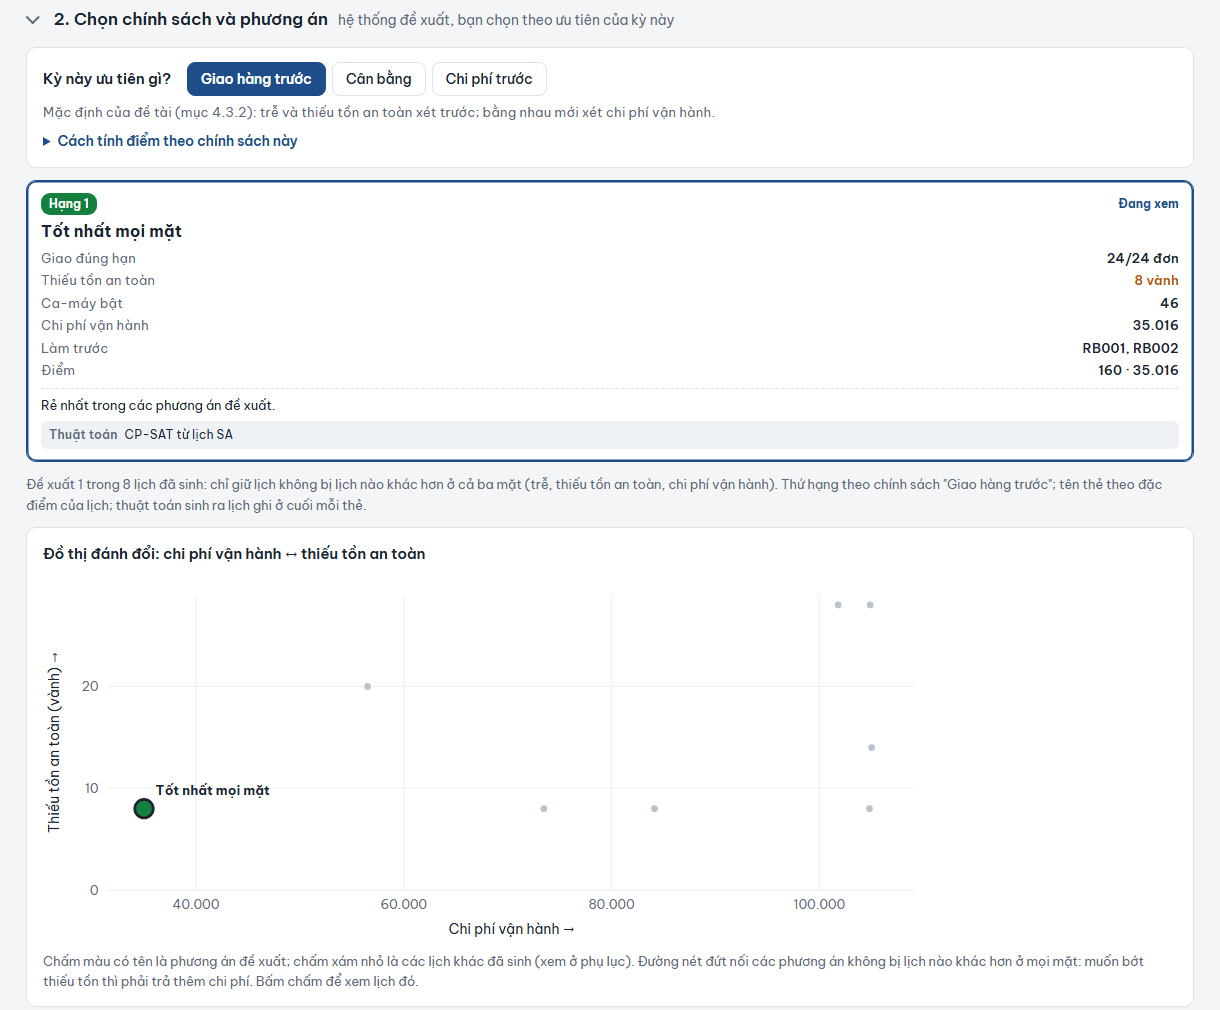
\includegraphics[height=6.3cm]{d2_phuong_an_2tuan.png}
\end{column}
\begin{column}{0.42\textwidth}
\scriptsize
\begin{itemize}\setlength{\itemsep}{0.35em}
  \item Chọn chính sách của kỳ: \textbf{giao hàng trước}, cân bằng, chi phí trước.
  \item Trong 8 lịch đã sinh chỉ còn \textbf{1 phương án không bị trội}: CP-SAT từ lịch SA --
        24/24 đơn đúng hạn, thiếu tồn 8 vành, 46 ca-máy.
  \item Thẻ phương án ghi điểm mạnh, các chỉ số và \textbf{thuật toán sinh ra nó}.
  \item Đồ thị đánh đổi chi phí vận hành $\leftrightarrow$ thiếu tồn an toàn; chấm xám là các lịch bị trội.
  \item Bấm chấm để xem lịch đó; so 2 phương án theo từng chỉ số và từng ca-máy chênh lệch.
\end{itemize}
\end{column}
\end{columns}
\end{frame}

\begin{frame}{Bàn điều độ: lịch chi tiết theo máy}
\framesubtitle{Phương án đề xuất, 4 ngày đầu của kỳ 2 tuần}
\centering
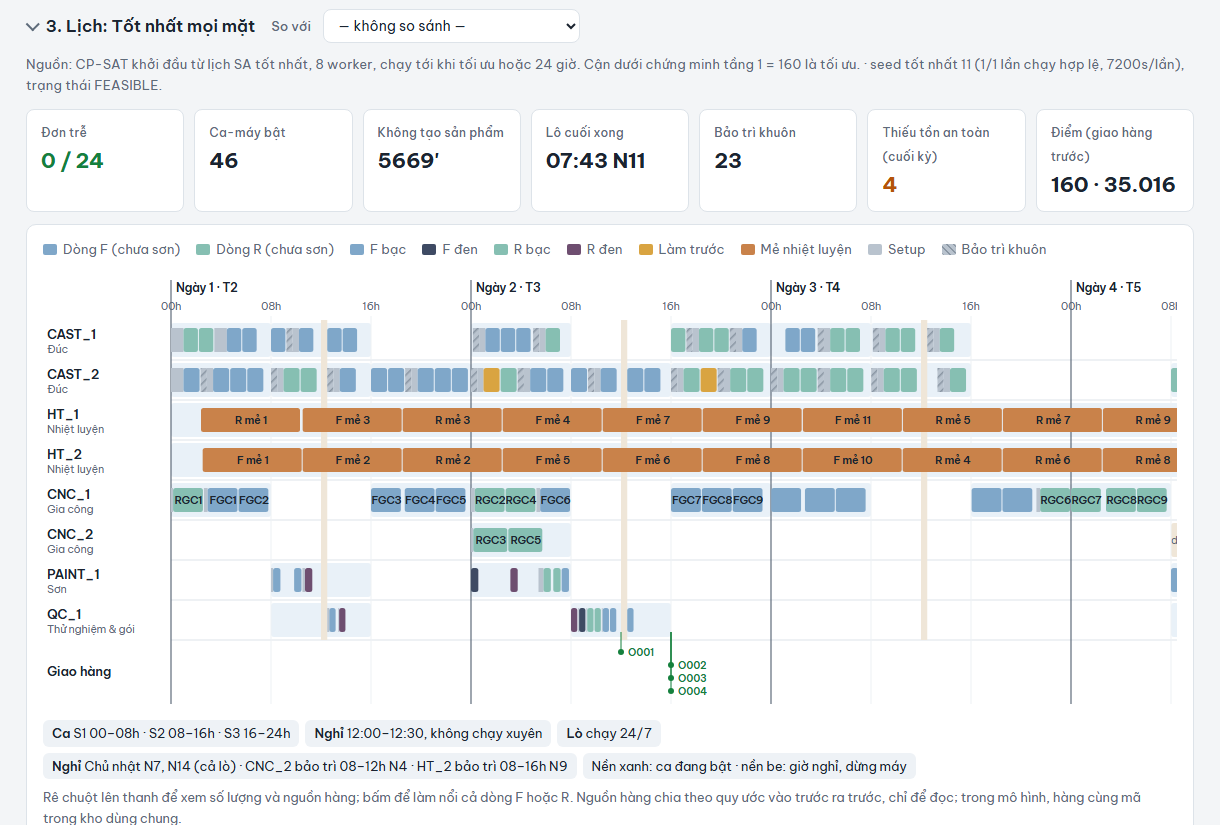
\includegraphics[width=0.84\linewidth,trim=0 110 0 100,clip]{d3_gantt_2tuan.png}\par
\vspace{0.2em}
{\scriptsize Ca đang bật, giờ nghỉ, dừng máy, setup, bảo trì khuôn, mẻ nhiệt luyện 8 giờ (cam), lượt làm trước, mốc giao hàng.
Kèm tồn BTP/thành phẩm đến cuối kỳ và mục ``vì sao xếp như vậy''.\par}
\end{frame}

\begin{frame}{Người lập kế hoạch trong vòng lặp}
\framesubtitle{Sửa tay một phương án, khoá phần cần giữ, để CP-SAT tối ưu lại phần còn lại}
\begin{columns}[T]
\begin{column}{0.48\textwidth}
\begin{block}{Sửa tay}
\scriptsize
\begin{itemize}\setlength{\itemsep}{0.2em}
  \item Kéo-thả lượt sang máy/thời điểm khác trên Gantt, hoặc đổi máy, thứ tự, giờ sớm nhất (có đường bàn phím).
  \item Mỗi thay đổi được \textbf{dựng lại theo cùng quy tắc xếp lịch}, kiểm tra độc lập và
        \textbf{chấm điểm trực tiếp} so với bản gốc; lỗi hiện bằng lời thường.
  \item Lượt không sửa giữ nguyên giờ cũ; bản sửa hợp lệ lưu thành \textbf{phương án mới}, được xếp hạng và chốt như phương án của bộ giải.
\end{itemize}
\end{block}
\end{column}
\begin{column}{0.48\textwidth}
\begin{block}{Tối ưu phần còn lại}
\scriptsize
\begin{itemize}\setlength{\itemsep}{0.2em}
  \item Khoá các lượt phải giữ, giữ các lượt đã sửa, đóng băng 24\,h / 48\,h đầu kỳ.
  \item CP-SAT tìm kiếm lân cận lớn \textbf{chỉ trên các lượt chưa khoá}, chạy nền 30\,s -- 5 phút.
  \item Bản sửa là phương án dự phòng: kết quả \textbf{không bao giờ kém hơn} bản sửa.
\end{itemize}
\end{block}
\vspace{-0.2em}
\begin{exampleblock}{Bộ 2 tuần}
\scriptsize Khoá 130/240 lượt, chạy 30\,s: chi phí vận hành \good{$-$1.370}, bớt 1 ca-máy.
\end{exampleblock}
\end{column}
\end{columns}
\vspace{0.3em}
\scriptsize Không cho sửa kỳ đã đóng; có hoàn tác/làm lại, cảnh báo khi rời trang chưa lưu, nhật ký thay đổi.
\end{frame}

% =====================================================================
\section{Đánh giá và kết luận}

\begin{frame}{Đối chiếu tiêu chí đánh giá}
\centering\scriptsize
\begin{tabular}{@{}L{4.3cm}L{9.6cm}@{}}
\toprule
Tiêu chí & Kết quả\\
\midrule
Lịch hợp lệ 100\% & \good{Đạt}: mọi lịch được xuất đều qua bộ kiểm tra độc lập; lần chạy không có lịch được báo rõ, không xuất lịch giả\\
Không trễ đơn trên bộ 2 tuần & \good{Đạt} (SA, GA, CP-SAT khởi đầu từ lịch SA)\\
Chứng minh chất lượng lời giải & \good{Một phần}: tầng 1 tối ưu đã chứng minh trên bộ 2 tuần; tầng 2 còn khoảng cách 51\%\\
Hiệu suất máy $\ge$ 90\% trong ca đã bật & \bad{Chưa đạt}: tăng từ 28--52\% lên \textbf{73,6\%}; tải tối thiểu thấp (ngay cả nhiệt luyện, công đoạn điểm nghẽn, chỉ 56--65\% ở bộ 2 tuần)
  $\Rightarrow$ cần định nghĩa lại theo công đoạn điểm nghẽn\\
Người lập kế hoạch chọn, sửa, chốt & \good{Đạt}: bàn điều độ trong sản phẩm, sửa tay + tối ưu phần còn lại, quyết định lưu CSDL kèm nhật ký\\
Thời gian giải chấp nhận được & Bộ 3 ngày: vài giây -- 60\,s; bộ 2 tuần: bước CP-SAT khoảng 10 phút; trạng thái giải luôn hiển thị\\
Diễn giải lịch (phụ trợ) & Một phần: đường đánh đổi, so 2 lịch, lý giải theo lịch; đường găng, độ nhạy \bad{chưa có}\\
Chất lượng trên benchmark công khai & \bad{Chưa đánh giá} (Taillard, Lawrence, Deliktaş đã có dữ liệu)\\
\bottomrule
\end{tabular}
\end{frame}

\begin{frame}{Giới hạn và kết luận}
\small
\begin{columns}[T]
\begin{column}{0.48\textwidth}
\begin{block}{Giới hạn}
\scriptsize
\begin{itemize}\setlength{\itemsep}{0.2em}
  \item Dữ liệu tổng hợp, mỗi quy mô một bộ, CP-SAT chạy 1 lần $\Rightarrow$ \textbf{thử nghiệm thăm dò}, chưa đủ kết luận thống kê.
  \item Trọng số mục tiêu là giả định chính sách, chưa quy đổi từ chi phí thật (7 biến thể trọng số: thứ hạng đầu không đổi).
  \item Chưa tái lập lịch khi sự cố phát sinh giữa chừng; chưa chạy benchmark công khai.
  \item CP-LNS và cuốn chiếu còn yếu ở quy mô 269 lượt.
\end{itemize}
\end{block}
\end{column}
\begin{column}{0.48\textwidth}
\begin{block}{Kết luận}
\scriptsize
\begin{itemize}\setlength{\itemsep}{0.2em}
  \item Không thuật toán đơn lẻ nào đủ; \textbf{phối hợp} luật $\to$ SA/GA/LNS $\to$ CP-SAT khởi đầu nóng cho lịch trội hơn mọi thành phần trên cả 2 bộ.
  \item Bộ kiểm tra độc lập + lọc Pareto + chính sách biến kết quả tối ưu thành \textbf{lịch hợp lý người quản lý tin dùng}.
  \item Người lập kế hoạch giữ quyền quyết định: chọn, sửa, chốt có lý do.
\end{itemize}
\end{block}
\vspace{-0.2em}
\begin{block}{Hướng tiếp theo}
\scriptsize
Benchmark Taillard/Lawrence (RPD) $\cdot$ tái lập lịch khi máy hỏng giữa kỳ $\cdot$ CP-LNS chỉ dựng các lượt được mở $\cdot$ đường găng, độ nhạy.
\end{block}
\end{column}
\end{columns}
\end{frame}

\begin{frame}[plain]
\centering
\vfill
{\usebeamercolor[fg]{title}\Huge Cảm ơn cô đã lắng nghe!\par}
\vspace{1em}
{\large Hỏi đáp và góp ý\par}
\vfill
\end{frame}

\end{document}
